\subsection{Alte und neue Familie}
Völlig überraschend starb am 19.
Juni 1926 August Högns Ehefrau Emma im Alter von 39 Jahren\footnote{
Dokument Nr. 109, Traueranzeige von August Högns Ehefrau Emma,
19.6.1926} an einem Gallendurchbruch. \footnote{Interview Nr. 20,
Gertraud von Molo, 23.11.2004, Absatz 4} Mitten aus dem Leben gerissen
hinterließ Emma Högn, die kurze Zeit davor Großmutter geworden war,
einen erst 14 Jahre alten Sohn. Das Tragische an Emmas Tod war, dass
sie an einer Krankheit starb, die schon zur damaligen Zeit hätte
behandelt werden können, wären die Symptome frühzeitig erkannt worden.
Mit nur 47 Jahren war August Högn Witwer geworden und musste sich nun
alleine um die Erziehung seines minderjährigen Sohns Gustl kümmern. Zur
Verrichtung der alltäglichen Arbeiten wurde auch deshalb die
Haushälterin Rosa Beischmied angestellt. \footnote{Interview Nr. 2,
Barbara Essigmann, 27.12.2002, Absatz 98}

\begin{center}
\begin{minipage}{5.992cm}
\begin{center}
\tablefirsthead{}
\tablehead{}
\tabletail{}
\tablelasttail{}
\begin{supertabular}{m{5.7920003cm}}

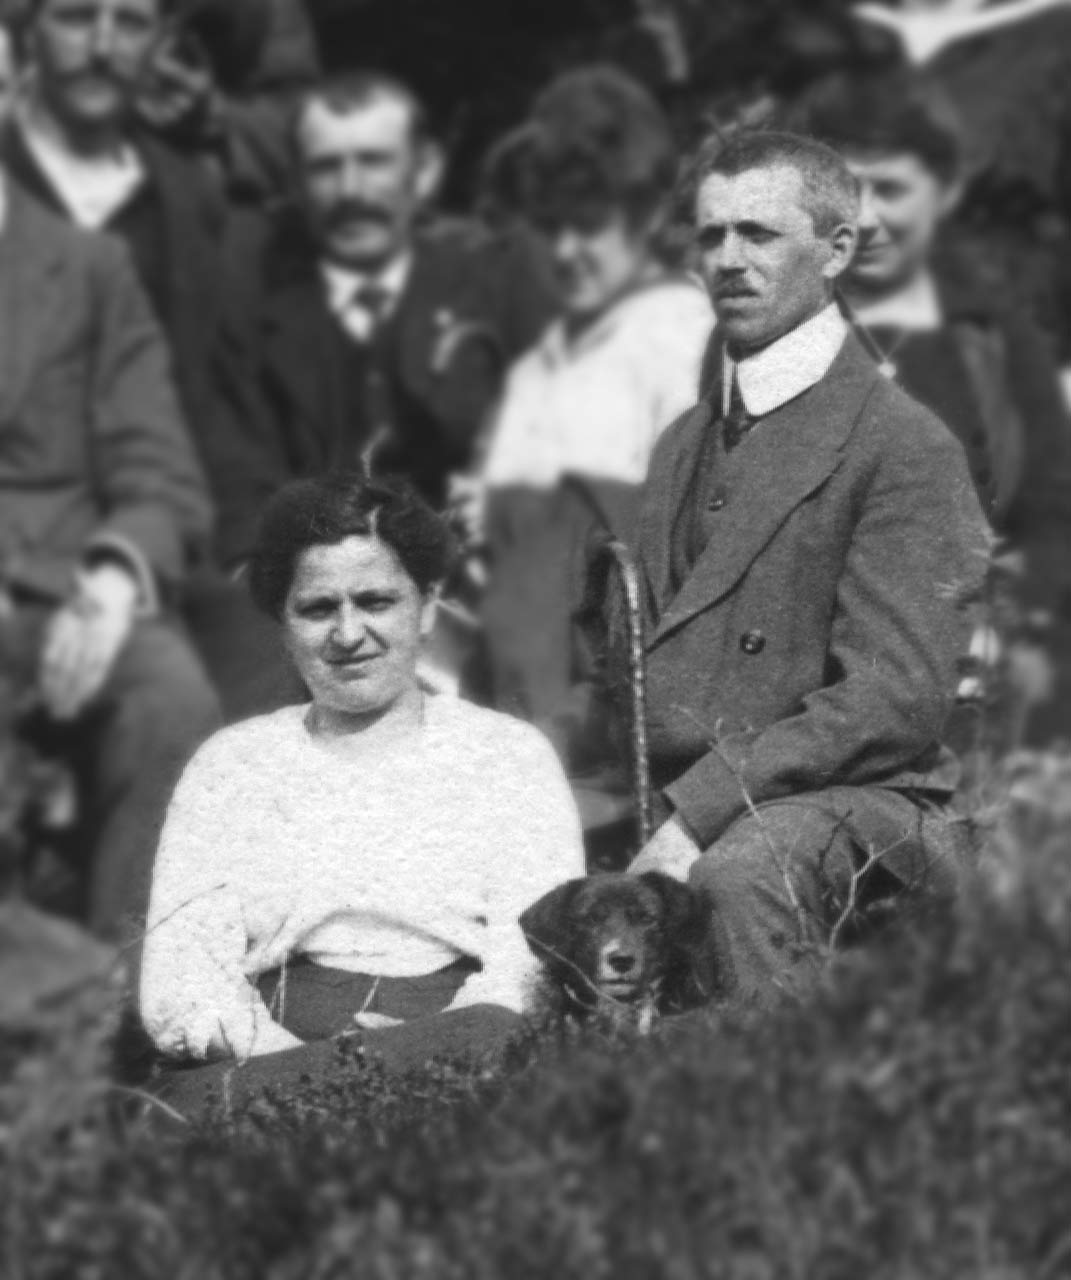
\includegraphics[width=5.609cm,height=6.705cm]{pictures/zulassungsarbeit-img024.jpg}

Emma und August Högn mit Jagdhund
„Treff“ bei einer Wanderung.\\
\end{supertabular}
\end{center}
\end{minipage}
\end{center}
Über den Zustand der Ehe Högns mit Emma ist kaum etwas bekannt.
Gerüchten zufolge soll Högns Ehefrau eine Affäre mit dem Nachbarn und
Kirchenchorsänger Rudolf Schwannberger gehabt haben.\footnote{
Interview Nr. 3, Ida Högn, 29.12.2002, Absatz 10} Ein möglicher Grund,
weshalb Högn kein zweites Mal geheiratet hat, könnte seine große Liebe
zu Emma gewesen sein. Ein weiterer Grund dafür dürfte auch seine
partnerschaftliche Beziehung zu Rosa Beischmied dargestellt haben, die
sich unweigerlich im Laufe der Jahre entwickelt hatte. Beide wurden als
eingespieltes Team beschrieben. \footnote{Interview Nr. 3, Ida Högn,
29.12.2002, Absatz 10} 35 Jahre lang begleitete Rosa Beischmied August
Högn bis zu seinem Tod und lebte mit ihm gemeinsam in derselben
Wohnung. \footnote{Interview Nr. 21, Lilo Leuze, 2.12.2004, Absatz 10;
Interview Nr. 20, Gertraud von Molo, 23.11.2004, Absatz 12} Je nach
Lebenslage unterstützte ihn die „Högn Rosl“, wie sie von einigen
Zeitzeugen genannt wurde, \footnote{Interview Nr. 2, Barbara Essigmann,
27.12.2002, Absatz 10, 76} etwa bei der Erziehung seines Sohnes, aber
auch beim Schuldienst, wenn zum Beispiel Högns Schüler Vitamintabletten
auf seine Anordnung hin, bei Rosa abholen mussten. \footnote{Interview
Nr. 6, Wilhelm Ederer, 2.1.2003, Absatz 34} Aber auch im Alter wurde
Högn von Rosa gepflegt, besonders nach seinem Schlaganfall.\footnote{
Dokument Nr. 73, Brief von August Högn an Stephan Leitner, 10.3.1961}
Nicht selbstverständlich und daher ebenso ein Indiz für das doch über
das rein Dienstliche hinausgehende Verhältnis zwischen Högn und
Beschmied war die Tatsache, dass Rosa Beischmieds „illegale“ Tochter
Mathilde, wie im Taufregister zu lesen ist, nach dem Tod ihrer
Großeltern in Högns Wohnung einziehen durfte. In der großen Wohnung im
Schulhaus erhielt sie ein eigenes Zimmer \footnote{Interview Nr. 19,
Mathilde Beischmied, 14.9.2004, Absatz 22} und fühlte sich von August
Högn sogar soweit akzeptiert, dass sie ihn heute als „Ersatzvater“
bezeichnet. \footnote{Interview Nr. 19, Mathilde Beischmied, 14.9.2004,
Absatz 18} Eine Anekdote, die Mathilde Beischmied in einem Interview
erzählte, mag vielleicht exemplarisch das gute und sehr
freundschaftliche Verhältnis Högns zu seiner Ziehtochter beleuchten und
Einblick ins damalige „Familienleben“ geben: Als Belohnung dafür, dass
die kleine Mathilde für Högn das Bier holte, bestand Högn darauf, dass
auch sie etwas von dem besorgten Getränk abbekam und fragte deshalb
ihre Mutter vorwurfsvoll: \zitat{„Kriegt sie heute kein
Bier?“ } \footnote{Interview Nr. 19, Mathilde Beischmied, 14.9.2004,
Absatz 6} Auch in der Funktion des Vaters, obwohl diese Bezeichnung
nicht zutrifft, zeigte sich Högn, als er für mehrere Jahre seine noch
schulpflichtige Enkelin Inge bei sich aufnahm. Als Grund, weshalb sie
zu ihrem Großvater kam, kann wohl die Trennung der ihrer Mutter Frieda
von ihrem ersten Ehemann und die neue Bekanntschaft mit ihrem späteren
Ehemann Dr. Karl Schlumprecht angesehen werden. \footnote{Interview Nr.
19, Mathilde Beischmied, 14.9.2004, Absatz 26} Da auch Högns Sohn Gustl
noch zu Hause wohnte, zählte Högns „neue Familie“ zusammen mit der
Enkelin Inge zeitweise sogar fünf Mitglieder.
